% このプリアンブルは削除しないでください。
% ファイル名はローマ字で「myouji_namae.pdf」のようにしてください。全て小文字で入力してください。
% 例:wakete_taro.pdf
% A4用紙2〜10ページで作成をお願いします。

%---------------- BEGIN -----------------
\documentclass[uplatex,11pt,a4paper,dvipdfmx]{jsarticle}
\usepackage[dvipdfm,truedimen,left=25truemm,right=25truemm,top=30truemm,bottom=30truemm]{geometry}
\pagestyle{empty}
%----------------- END ------------------

% もし jarticle をご使用の場合は、上記の BEGIN から END までをコメントアウトしてください。
% その上で、下記の BEGIN から END までと、\maketitle の直後のコメントアウトを解除してください。

%---------------- BEGIN -----------------
%\documentclass[11pt,a4paper]{jarticle}
%\usepackage[dvipdfm,left=25mm,right=25mm,top=30mm,bottom=30mm]{geometry}
%\pagestyle{empty}
%----------------- END ------------------

%%%%%%%% 以下のプリアンブルはご自由に編集してください。 %%%%%%%%
\usepackage[dvipdfmx]{graphicx}
\usepackage{amsfonts, amsmath, amsthm, amssymb}
\usepackage{mathtools}
\usepackage{tikz-cd}
\usepackage{here}
\usepackage{bm}
\usepackage{dynkin-diagrams}
\usepackage[all,knot]{xy}
\usepackage[backend=biber, style=alphabetic, sorting=nyt, url=false]{biblatex}
\addbibresource{../bib/double-affine-braid-group.bib} 
\AtBeginBibliography{\small}

\numberwithin{equation}{section}
\numberwithin{figure}{section}
\mathtoolsset{showonlyrefs=true}
\renewcommand{\theenumi}{\arabic{enumi}}
\renewcommand{\labelenumi}{(\theenumi) }
\providecommand{\MR}{\relax\ifhmode\unskip\space\fi MR }
%% Theorems
\theoremstyle{definition}
\newtheorem{theorem}{定理}[section]
\newtheorem{conjecture}[theorem]{予想}
\newtheorem{lemma}[theorem]{補題}
\newtheorem{proposition}[theorem]{命題}
\newtheorem{corollary}[theorem]{系}
\newtheorem{definition}[theorem]{定義}
\newtheorem{example}[theorem]{例}
\newtheorem{remark}[theorem]{補足}

%% Some operators
\DeclareMathOperator{\Hom}{\mathrm{Hom}}
\DeclareMathOperator{\Tor}{\mathrm{Tor}}
\DeclareMathOperator{\CHom}{\mathcal{H}\!\mathit{om}}
\DeclareMathOperator{\CTor}{\mathcal{T}\!\mathit{or}}
\DeclareMathOperator{\Auteq}{\mathrm{Auteq}}
\DeclareMathOperator{\Cone}{\mathrm{Cone}}
\DeclareMathOperator{\ev}{\mathrm{ev}}
\DeclareMathOperator{\id}{\mathrm{id}}
\DeclareMathOperator{\depth}{\mathrm{depth}}
\DeclareMathOperator{\Pic}{\mathrm{Pic}}
\DeclareMathOperator{\MCG}{\mathrm{MCG}}
\DeclareMathOperator{\PMCG}{\mathrm{PMCG}}
\DeclareMathOperator{\RHom}{\mathrm{RHom}}
\DeclareMathOperator{\Ker}{\mathrm{Ker}}
\DeclareMathOperator{\Image}{\mathrm{Im}}
\DeclareMathOperator{\Aut}{\mathrm{Aut}}
\DeclareMathOperator{\Inn}{\mathrm{Inn}}
\DeclareMathOperator{\Out}{\mathrm{Out}}
\DeclareMathOperator{\Supp}{\mathrm{Supp}}
\DeclareMathOperator{\SL}{\mathrm{SL}}
\DeclareMathOperator{\Spec}{\mathrm{Spec}}
\DeclareMathOperator{\Perf}{\mathrm{Perf}}
\DeclareMathOperator{\NS}{\mathrm{NS}}
\DeclareMathOperator{\Ext}{\mathrm{Ext}}
\DeclareMathOperator{\Hilb}{\mathrm{Hilb}}
\DeclareMathOperator{\res}{\mathrm{res}}
\DeclareMathOperator{\Ch}{\mathrm{Ch}}
\DeclareMathOperator{\coh}{\mathrm{coh}}
\DeclareMathOperator{\Fuk}{Fuk}
\DeclareMathOperator{\Ob}{Ob}
\DeclareMathOperator{\UConf}{UConf}
\DeclareMathOperator{\Aff}{Aff}
\DeclareMathOperator{\Diff}{Diff}


\newcommand{\nc}{\newcommand}

%% Calligraphic letters

\nc{\cF}{{\mathcal{F}}}
\nc{\cG}{{\mathcal{G}}}
\nc{\cH}{{\mathcal{H}}}

\nc{\cO}{{\mathcal{O}}}
\nc{\cU}{{\mathcal{U}}}
\nc{\cW}{{\mathcal{W}}}

%% Blackboard letters
\nc{\bA}{{\mathbb{A}}}
\nc{\bC}{{\mathbb{C}}}
\nc{\bP}{{\mathbb{P}}}
\nc{\bQ}{{\mathbb{Q}}}
\nc{\bR}{{\mathbb{R}}}
\nc{\bZ}{{\mathbb{Z}}}


\nc{\fsl}{{\mathfrak{sl}}}
\nc{\fgl}{{\mathfrak{gl}}}

\makeatletter
\newcommand*{\rom}[1]{\expandafter\@slowromancap\romannumeral #1@}
\makeatother

\title{Double affine braid group actions on derived categories of Kodaira fibers}    % ご自身の講演タイトル(申込み時に申請したもの)を記入してください。
\author{東京大学大学院 数理科学研究科 \\
荒井勇人 (Hayato ARAI) 
\footnote{E-mail:hayato@ms.u-tokyo.ac.jp}}    
%ご自身のお名前(漢字とローマ字両方)、正式な所属を記載するようにお願いします。
%その際、苗字のローマ字は全て大文字でお願いします。
\date{}    % ここは空欄のままでお願いします。

\begin{document}

\maketitle
%\thispagestyle{empty}    % jarticle をご使用の場合はここも解除してください。

\begin{abstract}   % ご自身のアブストラクトを記入してください。
    楕円曲線の退化として得られる特異曲線は小平ファイバーと呼ばれ、ADE型分類をもつ。ミラー対称性によりA型の小平ファイバーの導来圏にはA型の二重アファインブレイド群が自然に作用する。本講演では、この作用がSeidel--Thomasのspherical twistの変種として解釈でき、それを用いて他の型の小平ファイバーの導来圏にも対応する型の二重アファインブレイド群の作用が構成できることを説明する。
\end{abstract}

%%%%%%%% 以下の本文はご自由にお書きください。 %%%%%%%%

\section{導入}
本稿で扱う代数多様体は$\bC$上のものとする。
\subsection{楕円曲線と小平ファイバー}

平面上の三次式で表される代数曲線のうち、特異点を持たないものを\textbf{楕円曲線}という。
例えば曲線$y^2 = x^3 - x + 1$は楕円曲線である。$y^2 = x^3 + x^2$は三次式で定まるが、$f = y^2-x^3 - x^2$のJacobi行列$(-3x^2-2x, 2y)$は原点で$0$になるので特異点をもち、楕円曲線ではない。

\begin{figure}
    \centering
    \begin{minipage}{.3\textwidth}
        \centering
        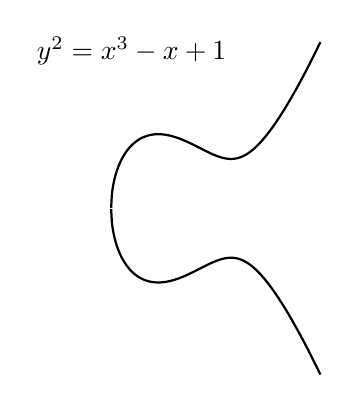
\begin{tikzpicture}[samples=300, scale=0.8]
            \draw(-1, 2.5) node{$y^2 = x^3-x+1$};
            \draw[thick,domain=-1.3247:2] plot(\x,{sqrt(\x^3-\x+1)});
            \draw[thick,domain=-1.3247:2] plot(\x,{-sqrt(\x^3-\x+1)});
        \end{tikzpicture}
        \caption{楕円曲線}
        \label{fig:fig1}
    \end{minipage}%
    \begin{minipage}{.3\textwidth}
        \centering
        \begin{tikzpicture}[samples=300, scale=0.8]
            \draw(-1.5, 2.5) node{$y^2 = x^3 + x^2$};
            \draw[thick, domain=-1:1.5, samples=100] plot(\x,{sqrt(\x+1)*(abs(\x))});
            \draw[thick, domain=-1:1.5, samples=100] plot(\x,{-sqrt(\x+1)*(abs(\x))});
        \end{tikzpicture}
        \caption{$\rom{1}_1$型小平ファイバー}
        \label{fig:fig2}
    \end{minipage}
    \begin{minipage}{.3\textwidth}
        \centering
        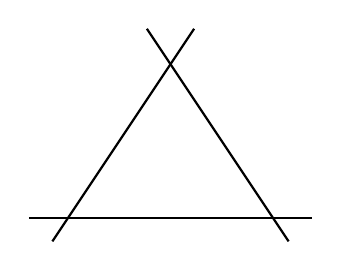
\begin{tikzpicture}[scale=0.3]
            % fiber
            \draw[thick] (-9,-1)--(-3,8);
            \draw[thick] (-10,0)--(2,0);
            \draw[thick] (1,-1)--(-5,8);
        \end{tikzpicture}
        \caption{$\rom{1}_3$型小平ファイバー}
        \label{fig:fig3}
    \end{minipage}%
\end{figure}
楕円曲線の族として得られる(非特異)曲面を楕円曲面という。
例えば、$t$をパラメータとする楕円曲線の族$y^2 = x^3 + x^2 + t$は楕円曲面である。
これは$t \neq 0$では楕円曲線だが、$t = 0$では特異曲線になる(退化する)。
より正確には、楕円曲面とは曲面$S$から曲線$C$への全射$\pi \colon S \to C$であって、有限個の$t \in C$を除いてファイバー$\pi^{-1}(t)$が楕円曲線になるようなもののことである。
いくつかのファイバーは特異点を持つかもしれないが、小平とN\'{e}ronは\textbf{相対的極小}という良いクラス\footnote{ファイバーに$(-1)$-曲線を含まない楕円曲面を相対的極小という。ファイバーに$(-1)$-曲線を含むときはそれらの曲線を1点に置き換える操作(ブローダウン)を繰り返して相対的極小にすることができる。}の楕円曲面に対しどのような特異ファイバーが現れるかを分類した。
それらを\textbf{小平ファイバー}といい、既約成分を頂点としその交点を辺としたグラフを考えることで(アファイン)Dynkin図形が得られ、それをもとに以下のように分類される。
\begin{enumerate}
    \item[$(\rom{1}_1)$] 1つの二重点を持つ有理曲線、Dynkin図形$A_1$
    \item[$(\rom{1}_n)$] $N \geq 2$本の$\bP^1$を$n$角形の形に並べたもの、アファインDynkin図形$\tilde{A}_{n-1}$
    \item[$(\rom{2})$] 1つの尖点を持つ有理曲線、$A_1$
    \item[$(\rom{3})$] 1点で重複度2で接する2本の$\bP^1$、$\tilde{A}_1$
    \item[$(\rom{4})$] 1点で交わる3本の$\bP^1$、$\tilde{A}_2$
    \item[$(\rom{1}^*_n)$] $4$本の$\bP^1$と$n+1 \geq 1$本の重複度$2$の$\bP^1$を既約成分を持つ曲線、$\tilde{D}_{n+4}$
    \item[$(\rom{2}^*)$] $9$本の重複度つき$\bP^1$を既約成分にもつ曲線、$\tilde{E}_8$
    \item[$(\rom{3}^*)$] $8$本の重複度つき$\bP^1$を既約成分にもつ曲線、$\tilde{E}_7$
    \item[$(\rom{4}^*)$] $7$本の重複度つき$\bP^1$を既約成分にもつ曲線、$\tilde{E}_6$
    \item[$({}_m\rom{1}_n)$] 重複度$m \geq 2$の$\rom{1}_n$型曲線
\end{enumerate}
本稿では初めに$A$型Dynkin図形に対応するもの、特に$n \geq 2$の$\rom{1}_n$型の小平ファイバーの導来圏について先行研究を紹介し、それらが$D$型と$E$型についてどのように拡張されるかを見ていく。
% TODO: 楕円曲線の例を図にする

\subsection{代数多様体の導来圏とホモロジー的ミラー対称性}
Abel圏に対し、その(有界)導来圏と呼ばれる三角圏が構成できる。
代数多様体$X$上の連接層のなすAbel圏$\coh X$の導来圏を$X$の\textbf{導来圏}といい、$D^b(X)$とあらわす。
$D^b(X)$の対象は連接層の複体であり、射の空間は$\Ext$群によって与えられる。
代数多様体の導来圏は1960年代にGrothendieckとVerdierによってSerre双対を一般的に記述する目的で導入され、現在では代数幾何学の重要な研究対象の1つとなっている。
ここではその重要性について、多様体の不変量としての側面と、ホモロジー的ミラー対称性における中心概念としての側面から説明する。

一般に空間$X$に対しその不変量を考えることは基本的である。
次元やコホモロジー群などが典型であり、代数多様体であればさらに$K$群、標準環などが挙げられるが、これらの多くが導来圏$D^b(X)$から計算できることが知られている。
また$\coh X$からは$X$の同型類そのものを復元できるが、$D^b(X)$については以下の2つの定理が示すように$X$を復元できる場合とできない場合がある。
\begin{theorem}[\cite{MR607081}]\label{thm:mukai}
    $X$をAbel多様体とし$\hat{X}$をその双対Abel多様体とする(これらは一般には同型ではない)。
    このとき三角圏としての同値$D^b(X) \cong D^b(\hat{X})$が存在する。
\end{theorem}
\begin{theorem}[\cite{MR1818984}]
    $X, Y$を非特異射影多様体とし、$X$の標準束$\omega_X$またはその双対束$\omega_X^\vee$が豊富な直線束だと仮定する。
    このとき$D^b(X)$と$D^b(Y)$が三角圏として同値ならば、$X\cong Y$である。
\end{theorem}
このように$D^b(X)$は$X$の幾何学について非常に多くの情報を持っている一方で、その全てを統制しているわけではない。
その意味で$X$の代わりに$D^b(X)$を考えることは双有理幾何学を考えることに似ている。
双有理幾何学と導来圏の間には実際に深いつながりがあることがわかっているが、ここでは省略する。


次にミラー対称性とは、ある空間$X$の代数幾何学と別の空間$M$のシンプレクティック幾何学の間に物理学の超弦理論に由来する不思議な関係があるという現象である。
この結び付きは例えば$X$内の有理曲線の数え上げ問題を$M$の周期積分に帰着して解決するなど、それまでの代数幾何学にはない物理学のアイデアに基づく新たな進展をもたらしてきた。
その背後にあるとされる最も強力な予想の1つが、Kontsevichの提唱した\textbf{ホモロジー的ミラー対称性}である。
\begin{conjecture}
    Calabi--Yau多様体$X$に対し別のCalabi--Yau多様体$M$が存在して、$X$の連接層の導来圏$D^b (X)$と$M$の深谷圏の導来圏$D^b \Fuk(M)$が(強化)三角圏として同値になる。
\end{conjecture}
ここで深谷圏$\Fuk(M)$とその導来圏$D^b \Fuk(M)$はシンプレクティック多様体$M$に対し定義されるもので、$D^b \Fuk(M)$の対象と射は大雑把にいうと$M$のLagrange部分多様体とその交差によって与えられる。
例えば$X$が楕円曲線$E$の場合、そのミラー$M$はトーラス$T$であり、$E$およびその閉点$x \in E$の構造層$\cO_E, \cO_x \in D^b(E)$がそれぞれ$T$上の緯線と経線に対応する \cite{MR1633036}。
このようにミラー対称性はまったく異なる種類の幾何学が等価であることを主張する非常に深い現象・予想であり、その記述には導来圏が現れる。
\begin{example}
    楕円曲線$E$とトーラス$T$のミラー対称性において、$\cO_E, \cO_x \in D^b(E)$は$T$上の曲線$\alpha, \beta \in D^b \Fuk(T)$に対応する(図\ref{fig:mirror-for-elliptic-curve})。$\sum_i \dim \Ext_{E}^i(\cO_E, \cO_x)=1$と$\# (\alpha \cap \beta) = 1$が一致していることは射の対応の帰結である。
    \begin{figure}[h]
        \begin{displaymath}
            \begin{tikzpicture}[samples=300, scale=0.8]
                % elliptic curve E
                \draw(-1, 2.5) node{$E$};
                \draw[thick,domain=-1.3247:2] plot(\x,{sqrt(\x^3-\x+1)});
                \draw[thick,domain=-1.3247:2] plot(\x,{-sqrt(\x^3-\x+1)});

                % point on E
                \filldraw[black] (0, 1) circle (3pt);
                \draw(0, 1.3) node[above]{$x$};

                % torus
                \draw(13, 2.5) node{$T$};
                % big square
                \draw[dashed] (5,-2)--(13,-2);
                \draw(9, -2) node{$>$};
                \draw[dashed] (5,2)--(13,2);
                \draw(9, 2) node{$>$};


                \draw[dashed] (5,-2)--(5,2);
                \draw(5, 0) node{\rotatebox{90}{$>>$}};
                \draw[dashed] (13,-2)--(13,2);
                \draw(13, 0) node{\rotatebox{90}{$>>$}};

                % horizontal lines
                \draw[ultra thick] (5, -1)--(13, -1);
                \draw(13, -1) node[right]{$\alpha$};

                % vertical lines
                \draw[ultra thick] (7, -2)--(7, 2);
                \draw(7, 2) node[above]{$\beta$};
            \end{tikzpicture}
        \end{displaymath}
        \caption{楕円曲線とトーラスのミラー対称性}
        \label{fig:mirror-for-elliptic-curve}
    \end{figure}
\end{example}
\subsection{Fourier--向井関手と捻り関手}
$X, Y$を非特異射影多様体とし、$p_X \colon X\times Y \to X, p_Y \colon X \times Y \to Y$を射影とする。
このとき、$X \times Y$の導来圏の対象$P \in D^b(X \times Y)$に対し関手
\begin{equation}
    \Phi^P \colon D^b(X) \xrightarrow{p_X^*} D^b(X \times Y) \xrightarrow{ - \otimes P} D^b(X \times Y) \xrightarrow{p_{Y*}} D^b(Y)
\end{equation}
を$P$を積分核とする\textbf{Fourier--向井関手(積分関手)}と呼ぶ。
ここで$p_X^*, p_{Y*}, - \otimes P$はそれぞれ逆像、順像、テンソル積(の導来関手)を意味する。
この名前は定理\ref{thm:mukai}のためにFourier変換の類似として向井により導入されたことによる。
以下の定理より、Fourier--向井関手は導来圏の間の関手、特に同値を調べる上で基本的な道具となる。
\begin{theorem}[\cite{MR1465519}]
    $X, Y$を非特異射影多様体とし、$\Phi \colon D^b(X) \to D^b(Y)$を充満忠実な三角関手とする。
    このとき$\Phi$はある積分核$P$によるFourier--向井関手$\Phi^P$と同型である。
\end{theorem}
導来圏$D^b(X)$の自己同値群$\Auteq D^b(X)$を、三角圏の構造を保つような$D^b(X)$の自己同値関手の同型類がなす群とする。
典型的な自己同値として、$X$の自己同型$f$による逆像$f^*(-)$、$X$上の直線束$L$によるテンソル積$(-)\otimes L$、および三角圏のシフト関手$(-)[1]$が常に存在し、これらの生成する$\Auteq D^b(X)$の部分群
\begin{equation}
    A(X) = \Aut(X) \ltimes \Pic(X) \times \bZ[1]
\end{equation}
の元は標準的な自己同値と呼ばれる。
以下の結果が基本的である。
\begin{theorem}[\cite{MR1818984}]\label{BO}
    $X$を非特異射影多様体とし、$X$の標準束$\omega_X$またはその双対束$\omega_X^\vee$が豊富な直線束だと仮定する。
    このとき$A(X) = \Auteq D^b(X)$である。
\end{theorem}
$A(X)$以外の自己同値を具体的に構成する方法として、SeidelとThomasは\cite{MR1831820}において捻り関手の概念を導入した。
\begin{theorem}[\cite{MR1831820}]
    $X$を$n$次元の非特異射影多様体とし、$E \in D^b(X)$を\textbf{球面対象}、すなわち\begin{equation}
        E \otimes \omega_X \cong E,\quad \Hom^i(E, E) = \begin{cases}
            \bC & i = \text{$0$ or $n$}, \\
            0   & \text{otherwise}
        \end{cases}
    \end{equation}を満たすものとする。
    このとき$P = \Cone(E^\vee \boxtimes E \xrightarrow{\ev} \cO_\Delta) \in D^b(X \times X)$を積分核とするFourier--向井関手$\Phi^P$は圏同値である。
    これを球面対象$E$に付随する\textbf{(球面)捻り関手}(spherical twist, twist functor)といい、$T_E$と書く。
\end{theorem}
定義より関手$T_E$について以下が得られる。これを$T_E$の定義だと思ってもよい。
\begin{corollary}
    $E \in D^b(X)$を球面対象とすると、任意の$F \in D^b(X)$について完全三角形
    \begin{equation}\label{eq:twist}
        \Hom^*(E, F) \otimes E \xrightarrow{\ev} F \to T_E (F) \xrightarrow{+1}
    \end{equation}
    が存在する。ここで$\ev$は自然なペアリング写像である。
\end{corollary}
この定義のモチベーションについて少し説明する。実曲面$\Sigma$上の閉曲線$\gamma$に対し、その\textbf{Dehn捻り}という$\Sigma$の自己同相が以下の図のように「$\gamma$に沿って$\Sigma$を切断し、180度捻って再接着する」ものとして定義されていた(図\ref{fig:dehn-twist})。


\begin{figure}[h]
    \centering
    \begin{displaymath}
        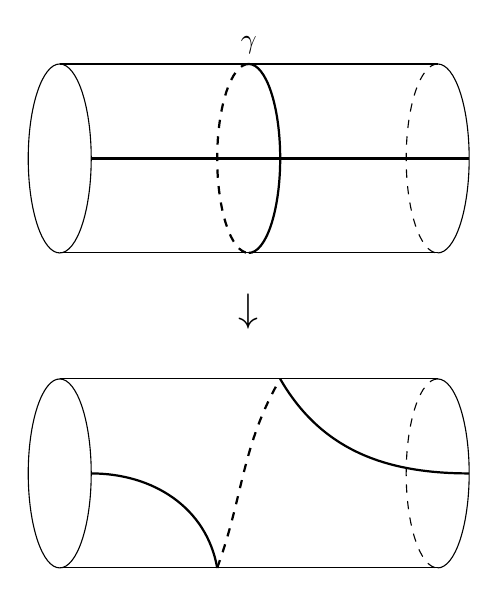
\begin{tikzpicture}[scale=0.8]
            \draw (0,0+5)--(6,0+5);
            \draw (0,3+5)--(6,3+5);

            \draw[thick] (0.5, 1.5+5)--(6.5, 1.5+5);

            \draw (0, 1.5+5) circle[x radius=0.5, y radius=1.5];

            \draw(6, 0+5)arc(-90:90:0.5 and 1.5);
            \draw[dashed](6, 3+5)arc(90:270:0.5 and 1.5);

            \draw[thick](3, 0+5)arc(-90:90:0.5 and 1.5);
            \draw[thick, dashed](3, 3+5)arc(90:270:0.5 and 1.5);


            % notation
            \draw(3, 3+5) node[above]{$\gamma$};

            \draw(3, -0.5+5) node[below]{\Large$\downarrow$};


            \draw (0,0)--(6,0);
            \draw (0,3)--(6,3);

            \draw (0, 1.5) circle[x radius=0.5, y radius=1.5];

            \draw(6, 0)arc(-90:90:0.5 and 1.5);
            \draw[dashed](6, 3)arc(90:270:0.5 and 1.5);

            \draw[thick](0.5, 1.5) to[out=0,in=100](2.5, 0);
            \draw[thick, dashed](2.5, 0) to[out=70,in=-120](3.5, 3);
            \draw[thick](3.5, 3) to[out=-60,in=180](6.5, 1.5);
        \end{tikzpicture}
    \end{displaymath}
    \caption{閉曲線$\gamma$に沿ったDehn捻り}
    \label{fig:dehn-twist}
\end{figure}



Seidel \cite{MR1743463}はこれを一般化し、$2n$次元シンプレクティック多様体$M$の中のLagrange球面$S^n$に対してDehn捻りを定義した。
ミラー対称性$D^b(X) \cong D^b \Fuk(M)$のもとではDehn捻りに対応して$D^b(X)$の自己同値が得られるが、これが捻り関手である。
もう少し詳しく述べると、
Lagrange球面$S^n \subset M$の、$D^b\Fuk(M)$の対象としての(次数付き)自己準同型環は
\begin{align}
    \Hom_{D^b\Fuk(M)}^*(S^n, S^n) & = HF^*(S^n, S^n)\otimes_\bR \bC
\end{align}
となり、Floerコホモロジー$HF^*(S^n, S^n)$は球面のコホモロジー$H^*(S^n, \bR)$と同型である。
よって、球面対象の2つ目の条件$$\Hom^i(E, E) = \begin{cases}
        \bC & i = 0, \dim X,   \\
        0   & \text{otherwise}
    \end{cases}$$は$E$の自己準同型環がLagrange球面$S^n$のそれと等しいことを意味する。
さらにSeidelは\cite{MR1978046}において、\eqref{eq:twist}と同様の完全三角形が導来深谷圏でのDehn捻りにおいても成り立つことを示した。
そこでこれらの性質をもとに($M$を登場させず)$D^b(X)$の言葉のみで代数的に定義されたものが捻り関手である。
\begin{example}
    \begin{enumerate}
        \item $E$を楕円曲線とすると、構造層$\cO_E$は$D^b(E)$の球面対象である。捻り関手$T_{\cO_E}$は標準的な自己同値ではない自己同値の例を与える。これは楕円曲線とトーラスのミラー対称性のもとで、$\cO_E$に対応するトーラスの緯線$\alpha$に沿ったDehn捻りに対応する(図\ref{fig:mirror-for-elliptic-curve})。
        \item $S$を非特異曲面とし、$\bP^1 \cong G \subset S$を$(-2)$-曲線とする。このとき$G$上の次数$a \in \bZ$の直線束$\cO_G(a)$を$S$上の層とみたものは、(Riemann--Rochの定理より)$D^b(S)$の球面対象である。
    \end{enumerate}
\end{example}
\subsection{ブレイド群}
ブレイド群(組み紐群, braid group)$B_n$は、$n$本の紐の絡まり方(組み紐)を元とし、それらを上下に接着することを演算として定義される群である。
ここで連続的に変形できる組み紐は同じ元とみなす。
例えば下図の組み紐は$B_3$の元の1つを表している。
\begin{figure}[h]
    \[
        \vcenter{\xy 0;/r2pc/:
        @={(0.5,-0.5),(0,0)}, @@{*{\vtwistneg}},(0,-2),\vtwist,
        @i@={(0,-1),(2,0),(2,-2)} @@{="save";"save"-(0,1),**@{-}}\endxy}
        \quad = \quad
        \vcenter{\xy 0;/r2pc/:
        @={(0.5,0),(0,-0.5),(0.5,-1)}, @@{*{\vtwistneg}},
        @i@={(0,0),(2,-1),(0,-2)} @@{="save";"save"-(0,1),**@{-}}\endxy}
    \]
    \caption{3本の紐からなる組紐}
    \label{fig:example-of-braid}
\end{figure}
$n$次対称群$S_n$は$n$本の線を持つあみだくじとその接着のなす群と思えるが、ブレイド群はそこに線の絡まり合いを許したようなものと考えられる。
対称群が隣り合う線の入れ替えによって生成されるのと同様に、ブレイド群は隣り合う紐の絡まり合いによって生成される。
ここでは紐$i$と$i+1$を入れ替える操作を$T_i$と書くことにする。
例えば図\ref{fig:example-of-braid}は$B_3$の中で$T_1T_2T_1 = T_2T_1T_2$が成り立つことを表している。
この関係式$T_iT_{i+1}T_i = T_{i+1}T_iT_{i+1}$を\textbf{ブレイド関係式}という。
また$|i-j| \geq 2$のとき明らかに$T_i$と$T_j$は可換である。
実はこれらの関係式のみで$B_n$が表されることが知られている。
\begin{theorem}[M.Artin]\label{thm:braid-group-as-artin-group}
    \begin{equation}
        B_n = \left\langle T_1, T_2, \dots, T_{n-1} \middle| \begin{split}
            &T_iT_{i+1}T_i = T_{i+1}T_iT_{i+1} \quad(1\leq i \leq n-2)\\
            &T_iT_j = T_jT_i\quad (|i-j| \geq 2)
        \end{split}\right\rangle {}_.
    \end{equation}
\end{theorem}
互換$(i, i+1)$を$s_i$とするとき$n$次対称群が
\begin{equation}
    S_n = \left\langle s_1, s_2, \dots, s_{n-1} \middle| \begin{split}
          &s_is_{i+1}s_i = s_{i+1}s_is_{i+1} \quad(1\leq i \leq n-2)\\
          &s_is_j = s_js_i\quad (|i-j| \geq 2), \quad s_i^2 = 1 \quad (1 \leq i \leq n-1)
      \end{split}\right\rangle
\end{equation}
と表示されることを思い出すと、ブレイド群は対称群の関係式のうち$s_i^2 = 1$を除いたものとみなせる。
特に自然な全射準同型$B_n \to S_n$が存在する。
このブレイド群には様々な一般化が考えられるが、ここでは2つの方向性について紹介する。

まず$n$本の紐を「平面上の$n$点の動き」とみなすと、ブレイド群の位相幾何的な解釈が得られる。
平面上の$n$点の(順序を無視した)配置のなす空間$\UConf_n(\bC)$を、$\bC^n$から対角集合$\{(x_i)_i \mid x_i \neq x_j \text{for some} i \neq j\}$を除いて座標の入れ替えによる対称群作用で割ったものとして定義する。
\begin{equation}
    \UConf_n(\bC) \coloneq (\bC^n \setminus \{(x_i)_i \mid x_i = x_j \text{ for some } i \neq j\}) / S_n.
\end{equation}
組み紐は空間$\UConf_n(\bC)$内のループとみなせ、ブレイド群は$\UConf_n(\bC)$の基本群として表される。
\begin{equation}
    B_n \cong \pi_1(\UConf_n(\bC)).
\end{equation}
そこで平面の代わりに別の空間を使うことで、同様の群を定義することができる。
例えばトーラス$T^2$をとれば\textbf{楕円ブレイド群}$B^{Ell}_n$が得られる。
これは隣り合う点を入れ替える操作$T_1, \dots, T_{n-1}$と、点を緯線または経線に沿って一周させる操作$X_1, \dots, X_n, Y_1, \dots, Y_n$によって生成される(図\ref{fig:generator-for-elliptic-braid-group})。
\begin{figure}[h]
    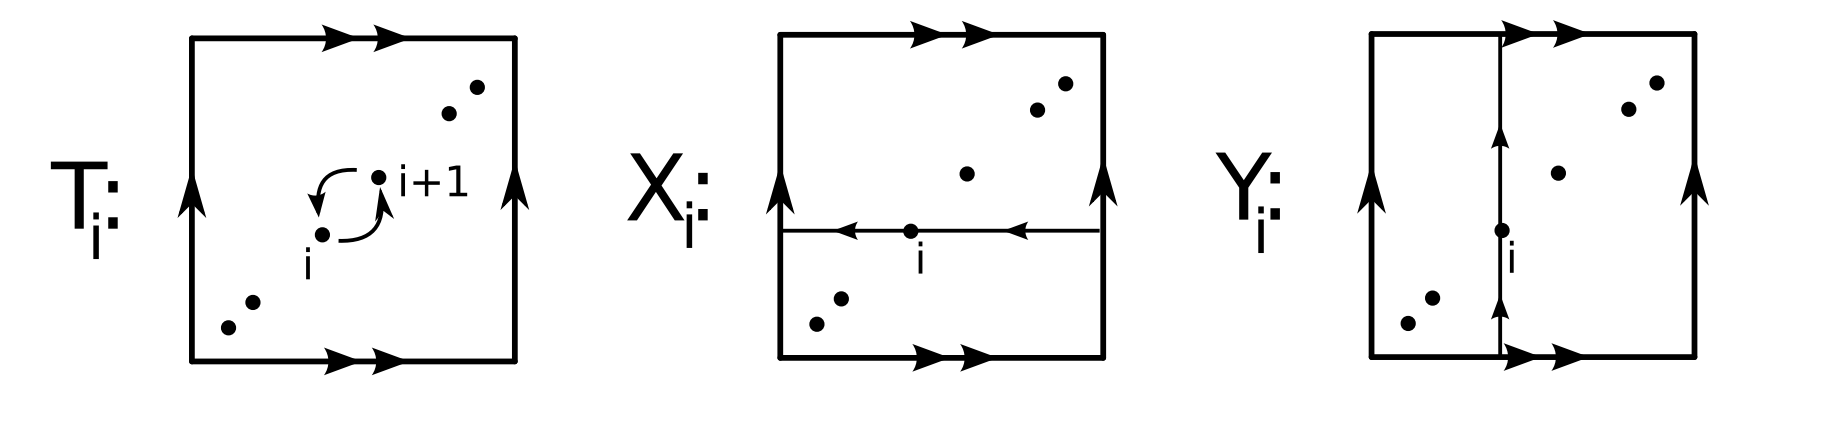
\includegraphics[width=150mm]{../images/elliptic_braid_group.png}
    \caption{$B^{Ell}_n$の生成元(\cite{MR2507111}より引用)}
    \label{fig:generator-for-elliptic-braid-group}
\end{figure}

また対称群$S_n$が$A_{n-1}$型ルート系のWeyl群であることを思い出すと、より一般のルート系に対して定理\ref{thm:braid-group-as-artin-group}のような形で組み合わせ論的にブレイド群やその変種を定義することができる。
\begin{definition}
    $R$を既約有限ルート系とし$\{\alpha_1, \dots, \alpha_n\} \subset R$を基底の1つとする。
    $R$のWeyl群$W$は$\alpha_i$に対応する鏡映$s_i$たちで生成され、鏡映$s_i$は$s_i^2=1$と(適切な)ブレイド関係式を満たす。そこで$T_1, \dots, T_n$を生成元とし$s_i$の関係式のうち$s_i^2=1$を除いたものを関係式として定まる群を\textbf{ブレイド群}といい、$B$と書く。
    $B$は$R$の基底の取り方によらない。
\end{definition}
ユークリッド空間$V$上の有限ルート系$R$があると、そこからアファインルート系$R^{a}$が$\{\alpha + n \delta \in \Aff(V) \mid \alpha \in R, n \in \bZ\}$により定まる。
ここで$\Aff(V)$は$V$上のアファイン関数のなすベクトル空間で、$\delta$は定数関数$1$である。
$R$の基底$\{\alpha_1, \dots, \alpha_n\} \subset R$は自然に$R^{a}$の基底$\{\alpha_0, \dots, \alpha_n\} \subset R^{a}$を与える。
このとき$R^{a}$のWeyl群$W^{a}$は鏡映$s_0, \dots, s_n$で生成され、特に$W = \langle s_1, \dots, s_n\rangle \subset W$である。
さらに以下のような表示も知られている。
\begin{proposition}
    $R$のコルート格子を$Q^\vee \subset V$とすると、平行移動により$Q^\vee \subset W^{a}$とみなせる。そして$W^{a} \cong W \ltimes Q^\vee$である。右辺は$R$の\textbf{アファインWeyl群}と呼ばれる。
\end{proposition}
コルート格子$Q^\vee$はコウェイト格子$P^\vee$の部分格子だから、$W^{ae} = W \ltimes P^\vee$と定めると$W^{a}$を含む群$W^{ae}$が得られる。これを$R$の\textbf{拡大アファインWeyl群}と呼ぶ。
これらのWeyl群から鏡映の関係式$s_i^2 = 1$を忘れることで\textbf{アファインブレイド群}$B^{a}$と\textbf{拡大アファインブレイド群}$B^{ae}$が定義される。
これらの群は$B, Q^\vee \subset B^{a}$や$B, P^\vee \subset B^{ae}$という部分群を持ち、それらによって生成される。
\begin{equation}
    B^{a} = \langle B, Q^\vee \rangle, \quad B^{ae} = \langle B, P^\vee \rangle.
\end{equation}
$B^{ae}$にさらにウェイト格子$P$を付け加えて生成されるのが、\textbf{二重アファインブレイド群}$B^{d}$である。
\begin{equation}
    B^{d} = \langle B, P^\vee, P\rangle.
\end{equation}
以上の厳密な定義には触れないが、右辺の生成元の間の関係式は明示的に与えられることを述べておく。
これらのブレイド群はMacdonald予想に関連してCherednikが導入した二重アファインHecke環(double affine Hecke algebra, DAHA)の理論に現れるものである。

\begin{remark}\label{remark:gl-braid-group}
    $A_n$型既約有限ルート系は単純Lie代数$\fsl_{n+1}$に対応するが、
    $\fsl_{n+1}$の代わりに簡約Lie代数$\fgl_{n+1}$に対応する二重アファインブレイド群を定義することもできる。
    この場合ブレイド群$B$は$A_n$型のまま、$P$や$P^\vee$が$\fsl_{n+1}$のものから$\fgl_{n+1}$のものに置き換えられる。
    \textbf{得られる二重アファインブレイド群$B^d$は楕円ブレイド群$B^{Ell}_n$と同型になる}ことが知られている。
\end{remark}


最後にブレイド群と導来圏の関係について述べる。
SeidelとThomasは良い条件を満たす球面対象の族から導来圏への忠実なブレイド群作用が誘導されることを示した\cite{MR1831820}。
\begin{theorem}[\cite{MR1831820}]
    $X$を非特異射影多様体とし、$E_1, \dots, E_m \in D^b(X)$を球面対象であって以下の条件を満たすものとする。
    \begin{equation}
        \sum_k\dim_\bC\Hom^k(E_i, E_j) = \begin{cases}
            1 & |i-j| = 1,    \\
            0 & |i-j| \geq 2.
        \end{cases}
    \end{equation}
    このとき生成元$T_i$を捻り関手$T_{E_i}$に送るような\textbf{単射}群準同型$B_{m+1} \to \Auteq D^b(X)$が存在する。
\end{theorem}




\section{主結果}
筆者はSeidel--Thomasの捻り関手を用いて新たな自己同値$H_E$を導入した。
\begin{theorem}[\cite{2023arXiv230212501A}]
    $\pi \colon X \to T$を非特異射影多様体の間の平坦射とし、$i \colon X_0 = \pi^{-1}(0) \to X$をファイバーとする。
    また$E \in D^b(X_0)$を、$i_*E \in D^b(X)$が球面対象になるような対象とする。
    このとき以下の図式を可換にするような同値$H_E \colon D^b(X_0) \to D^b(X_0)$が$E$と$i$から構成できる。
    \begin{equation}
        \begin{tikzcd}
            D^b(X_0) \arrow[r,"i_*"]\arrow[d, "H_E"'] & D^b(X) \arrow[d,"T_{i_*E}"]\\
            D^b(X_0) \arrow[r, "i_*"]& D^b(X).
        \end{tikzcd}
    \end{equation}
\end{theorem}

これを楕円曲面$\pi \colon S \to C$に適用する。$i \colon F = \pi^{-1}(0) \hookrightarrow S$を既約成分が2個以上ある特異ファイバーとすると、その既約成分$G \subset F$は$S$の$(-2)$-曲線となる。
よって$G \cong \bP^1$上の次数$a$の直線束$\cO_G$は$D^b(S)$の球面対象を与える。
上の定理より、$D^b(S)$の自己同値$T_{\cO_G(a)}$と整合的な$D^b(F)$の自己同値$H_{\cO_G(a)}$が得られる。
捻り関手はDehn捻りの対応物だったが、$F$が$\rom{1}_n$型の場合この$H_{\cO_G(a)}$は実曲面の\textbf{半捻り}という操作の対応物となる。
具体的に説明しよう。
$n \geq 2$とし、$F_n$を$\rom{1}_n$型の小平ファイバーとする。
$F_n$のミラー多様体は$n$点穴あきトーラス$T_n$である。

\begin{theorem}[\cite{MR3663596}]
    $\cW(T_n)$を$T_n$の巻深谷圏(wrapped Fukaya category)とすると、三角圏の同値$D^b(F_n) \cong D^b(\cW(T_n))$がある。
\end{theorem}
これにより$E \in D^b(F_n)$に対応する曲線を$\gamma_E$としよう。
\begin{example}\label{correspondence_of_objects}
    $n=3$とする。$F_3$の既約成分を$G_1, G_2, G_3$とし、それらの上にある非特異点を$x_1, x_2, x_3$とする。
    このとき直既約対象$\cO_{F_3}, \cO_{G_1}, \cO_{G_1}(-1), \cO_{x_1}$などに対応する$T_3$上の曲線は図\ref{fig:mirror-figure}のような曲線である。
    ただし白い丸は$T_3$の$3$つの穴を表す。
    \begin{figure}[h]
        \centering
        \begin{displaymath}
            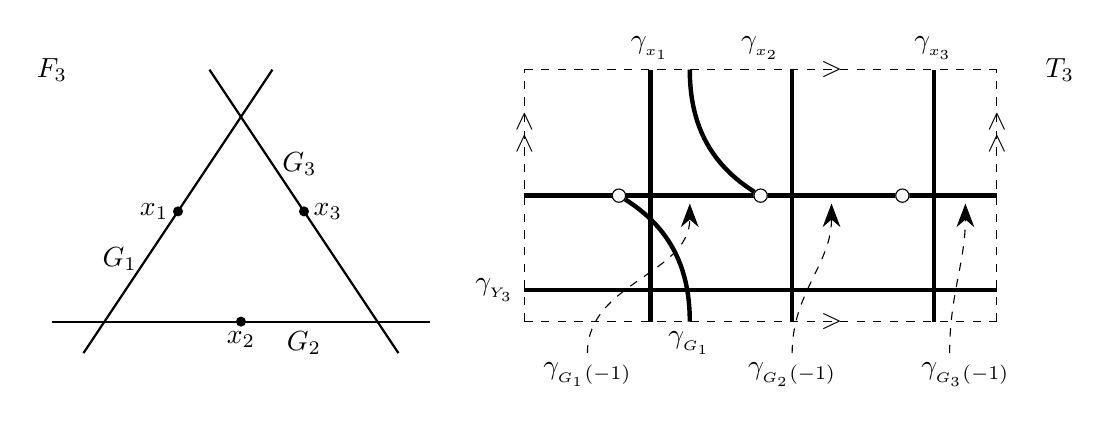
\begin{tikzpicture}[scale = 0.4]
                % fiber
                \draw(-10, 8) node{$F_3$};
                \draw[thick] (-9,-1)--(-3,8);
                \draw[thick] (-10,0)--(2,0);
                \draw[thick] (1,-1)--(-5,8);

                % points
                \filldraw[black] (-6, 3.5) circle (4pt);
                \filldraw[black] (-4, 0) circle (4pt);
                \filldraw[black] (-2, 3.5) circle (4pt);

                \draw(-6, 3.5) node[left]{$x_1$};
                \draw(-4, 0) node[below]{$x_2$};
                \draw(-2, 3.5) node[right]{$x_3$};

                % components
                \draw(-7, 2) node[left]{$G_1$};
                \draw(-2, 0) node[below]{$G_2$};
                \draw(-3, 5) node[right]{$G_3$};

                % big square
                \draw(22, 8) node{$T_3$};
                \draw[dashed] (5,0)--(20,0);
                \draw(14.75, 0) node{$>$};
                \draw[dashed] (5,0)--(5,8);
                \draw(5, 6) node{\rotatebox{90}{$>>$}};
                \draw[dashed] (5,8)--(20,8);
                \draw(14.75, 8) node{$>$};
                \draw[dashed] (20,0)--(20,8);
                \draw(20, 6) node{\rotatebox{90}{$>>$}};

                % horizontal lines
                \draw[ultra thick] (5, 1)--(20, 1);
                \draw[ultra thick] (5, 4)--(20, 4);
                \draw(5, 1) node[left]{$\gamma_{\cO_{Y_3}}$};

                % vertical lines
                \draw[ultra thick] (8+1, 0)--(8+1, 8);
                \draw(8+1, 8) node[above]{$\gamma_{\cO_{x_1}}$};
                \draw[ultra thick] (12.5+1, 0)--(12.5+1, 8);
                \draw(12.5, 8) node[above]{$\gamma_{\cO_{x_2}}$};
                \draw[ultra thick] (17+1, 0)--(17+1, 8);
                \draw(17+1, 8) node[above]{$\gamma_{\cO_{x_3}}$};

                % curves
                \draw[ultra thick] (8, 4) to[out=-30,in=90] (10.25, 0);
                \draw[ultra thick] (10.25, 8) to[out=-90,in=150] (12.5, 4);
                \draw(10.25, 0) node[below]{$\gamma_{\cO_{G_1}}$};
                % punctures
                \foreach \u in {8, 12.5, 17}
                    {
                        \filldraw[white] (\u, 4) circle (6pt);
                        \draw[black] (\u, 4) circle (6pt);
                    }

                % O_G(-1)
                \draw[dashed, -{Stealth[length=3mm]}] (7, -1) to[out=90, in=-90] (10.25, 3.75);
                \draw(7, -1) node[below]{$\gamma_{\cO_{G_1}(-1)}$};
                \draw[dashed, -{Stealth[length=3mm]}] (13.5, -1) to[out=90, in=-90] (14.75, 3.75);
                \draw(13.5, -1) node[below]{$\gamma_{\cO_{G_2}(-1)}$};
                \draw[dashed, -{Stealth[length=3mm]}] (18.5, -1) to[out=90, in=-90] (19, 3.75);
                \draw(19, -1) node[below]{$\gamma_{\cO_{G_3}(-1)}$};
            \end{tikzpicture}
        \end{displaymath}
        \caption{$D^b(F_n)$の対象と$T_3$上の曲線の対応}
        \label{fig:mirror-figure}
    \end{figure}
\end{example}

また$T_n$の写像類群$\MCG(T_n)$\footnote{正確には深谷圏の$\bZ$次数構造と整合する次数付き写像類群$\widetilde{\MCG}(T_n)$を考える必要がある。}は$\cW(T_n)$への自然な作用を通じて$D^b(F_n)$へ作用する。
$\MCG(T_n)$は緯線や経線に沿ったDehn捻りと、2つの穴を結ぶ曲線に沿った半捻りという操作で生成される \cite{MR1805936}。
例えば図\ref{fig:mirror-figure}の$\gamma_{\cO_{G_1}(-1)}$は穴を結ぶ曲線で、半捻りとは図\ref{fig:half-twist}の操作である。
\begin{figure}[h]
    \begin{displaymath}
        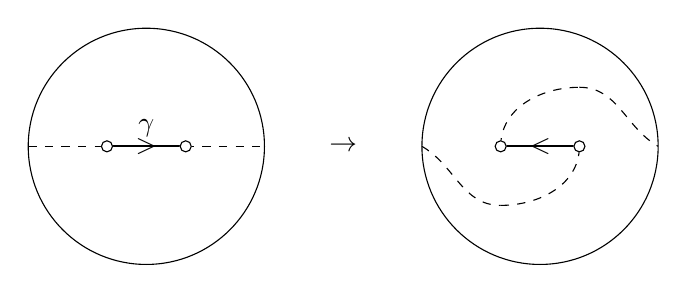
\begin{tikzpicture}
            \draw (0, 1.5) circle[radius=1.5];
            \draw[thick] (-0.5, 1.5)--(0.5, 1.5);
            \draw(0, 1.5) node{$>$};
            \draw[dashed] (-1.5, 1.5)--(-0.5, 1.5);
            \draw[dashed] (0.5, 1.5)--(1.5, 1.5);

            \foreach \u in {-0.5, 0.5}
                {
                    \filldraw[white] (\u, 1.5) circle (2pt);
                    \draw[black] (\u, 1.5) circle (2pt);
                }
            \draw(0, 1.5) node[above]{$\gamma$};

            \draw(2.5, 1.5) node{$\rightarrow$};

            \draw (0+5, 1.5) circle[radius=1.5];
            \draw[thick] (-0.5+5, 1.5)--(0.5+5, 1.5);
            \draw(5, 1.5) node{$<$};


            \draw[dashed](-1.5+5, 1.5) to[out=-30,in=180](-0.5+5, 0.75);
            \draw[dashed](-0.5+5, 0.75) to[out=0,in=-90](0.5+5, 1.5);

            \draw[dashed](-0.5+5, 1.5) to[out=90,in=180](0.5+5, 2.25);
            \draw[dashed](0.5+5, 2.25) to[out=0,in=150](1.5+5, 1.5);


            \foreach \u in {-0.5, 0.5}
                {
                    \filldraw[white] (\u+5, 1.5) circle (2pt);
                    \draw[black] (\u+5, 1.5) circle (2pt);
                }
        \end{tikzpicture}
    \end{displaymath}
    \caption{曲線$\gamma$に沿った半捻り}
    \label{fig:half-twist}
\end{figure}
\begin{theorem}[\cite{2023arXiv230212501A}]
    $\rom{1}_n$型小平ファイバー$F_n$について、$H_{\cO_G(a)} \in \Auteq D^b(F_n)$は$\gamma_{\cO_G(a)}$に沿った$T_n$の半捻りが誘導する自己同値である。
\end{theorem}
この結果を踏まえ、$H_{\cO_G(a)}$を$\cO_G(a)$に沿った\textbf{半捻り関手}と呼ぶことにする。
他の型の小平ファイバーにも半捻り関手$H_{\cO_G(a)}$を定義することができるが、\textbf{ミラー対称性は}$\rom{1}_n$\textbf{型の場合にしか知られていない}ため同じ手法で$H_{\cO_G(a)}$を調べることはできない。

一方、写像類群$\MCG(T_n)$は楕円ブレイド群$B^{Ell}_n = \pi_1(\UConf_n(T^2))$と以下のように関係する。
$T^2$上の$n$点集合$P_n = \{t_1, \dots, t_n\}$を固定し、$T_n = T^2 \setminus P_n$だとする。
$\Diff(T^2)$を$T^2$の自己微分同相群、$\Diff(T^2, P_n)$を$P_n$を集合として保つような自己微分同相のなす部分群とする。
後者は$\Diff(T_n)$と同一視できること、$\pi_0(\Diff) = \MCG$であることに注意する。
$\varphi \in \Diff(T^2)$を$\varphi(P_n) \in \UConf_n(T^2)$へ送る写像はファイバー束$\Diff(T^2, P_n) \hookrightarrow \Diff(T^2) \twoheadrightarrow \UConf_n(T^2)$を与え、そのホモトピー長完全列から準同型$\delta \colon B^{Ell}_n \to \MCG(T_n)$を得る。

以上より$B^{Ell}_n$の$D^b(F_n)$への作用が得られ、$B^{Ell}_n$の生成元$T_i, X_i, Y_i$のうち$T_i$は半捻り関手$H_{\cO_{G_i}(-1)}$として作用することが具体的な計算でわかる(図\ref{fig:generator-for-elliptic-braid-group}や図\ref{fig:mirror-figure}を参照)。
また$X_i, Y_i$の作用も具体的な捻り関手や直線束によるテンソル積関手を用いて表せる。
補足\ref{remark:gl-braid-group}より$B^{Ell}_n$は$A$型の二重アファインブレイド群と見なすことができるから、同様の群作用が$D$型や$E$型Dynkin図形に対応する小平ファイバーの導来圏にあるかどうかという問題が考えられる。
以下が主結果である。

\begin{theorem}[A.]
    $F$が$D$型または$E$型のDynkin図形に対応する小平ファイバーのとき、そのDynkin図形に対応するルート系が定める二重アファインブレイド群$B^d = \langle B, P^\vee, P\rangle$が$D^b(F)$に作用する。
    $B$の作用は半捻り関手で、$P^\vee$と$P$の作用は捻り関手と直線束によるテンソル積で与えられる。
\end{theorem}
\begin{remark}
    $A$型Dynkin図形を持つ小平ファイバーで$\rom{1}_n$型以外のものでも、ほとんど同様に二重アファインブレイド群や$\MCG(T_n)$の作用を構成できる。
\end{remark}






















\printbibliography[title=参考文献]




\end{document}
